%%% IMPORTANT: COMPILE WITH XeLaTeX

\documentclass[12pt]{article}
%All packages used this far
%\usepackage[latin1]{inputenc}
%\usepackage{times}
%\usepackage{logicproof}
%\usepackage{enumerate}
%\usepackage{cancel}
\usepackage{fullpage} % required for this template
%\usepackage{color}
%\usepackage{qtree}
%\usepackage{amsmath}
\usepackage{fontspec} % required for this template
%\usepackage{amssymb}
%\usepackage{amsthm}
%\usepackage{prooftrees}
\usepackage{tikz}
%\usepackage{circuitikz}
%\usepackage{colortbl}
%\usepackage{karnaugh-map}
%\usepackage[margin=1in]{geometry} % not sure if useful
%\usepackage{indentfirst}
%\usepackage{pgfplots}
%\usepackage{xcolor}
%\usepackage{arydshln}
%\usepackage{hyperref}

% Tikz libraries
%\usetikzlibrary{positioning}
%\usetikzlibrary{shapes.multipart}
%\usetikzlibrary{decorations.text}
%\usetikzlibrary{datavisualization}
%\usetikzlibrary{datavisualization.formats.functions}
%\usetikzlibrary{patterns}
%\usetikzlibrary{arrows.meta}
%\usetikzlibrary{quotes}
%\usetikzlibrary{automata}


\setromanfont{Times New Roman}
\setsansfont{Helvetica}

%Symbols that might be necessary
%\DeclareMathSymbol{@}{\mathord}{letters}{"3B}
%\newcommand{\powerset}{\raisebox{.15\baselineskip}{\Large\ensuremath{\wp}}}

\begin{document}

\noindent
Universidade Federal do Rio Grande do Sul \hfill Instituto de Informática \newline 
INF01009 -- Computação Gráfica \hfill 2023/1 \newline
Aluno \hfill Pedro Company Beck -- 00324055
\rule{\linewidth}{1.pt}

\begin{center}
	\LARGE\textbf{Assignment 1} 
\end{center}

\begin{itemize}
\item[(a)]
When the program is launched, the following interface shows up:
\begin{center}
	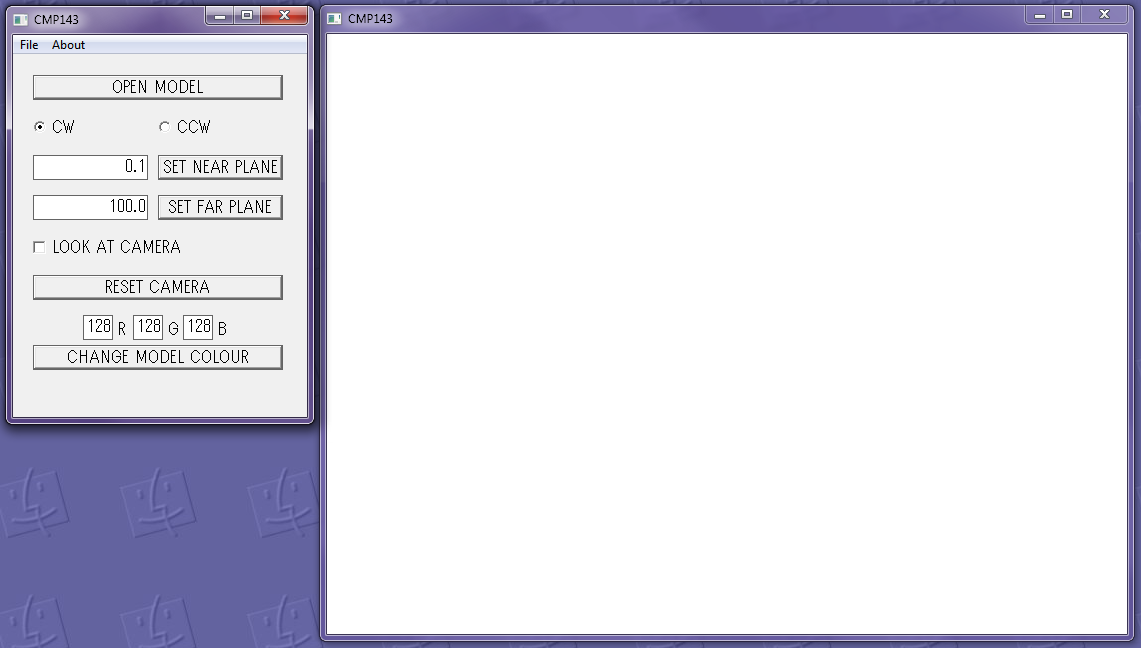
\includegraphics[scale=0.5]{1.png}
\end{center}
The interface with the commands was developed using the library \texttt{Windows.h}. The program does not load any models by default, they have to be loaded by clicking the ``OPEN MODEL'' button.

When the button is clicked, a Windows file picker dialog appears and the user can pick any model file with the \texttt{.in} format, as shown below:
\begin{center}
	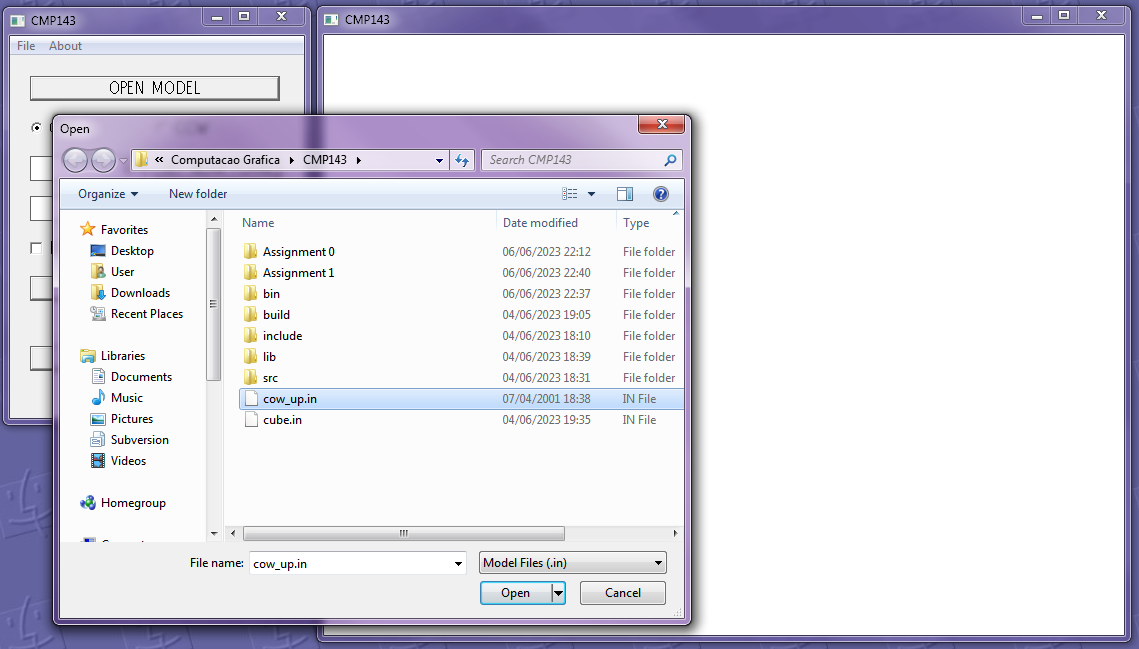
\includegraphics[scale=0.5]{2.png}
\end{center}
In this example, the \texttt{cow\_up.in} file was loaded.

After loading the cow model, it's shown at the middle of the right window on a grey colour.
\begin{center}
	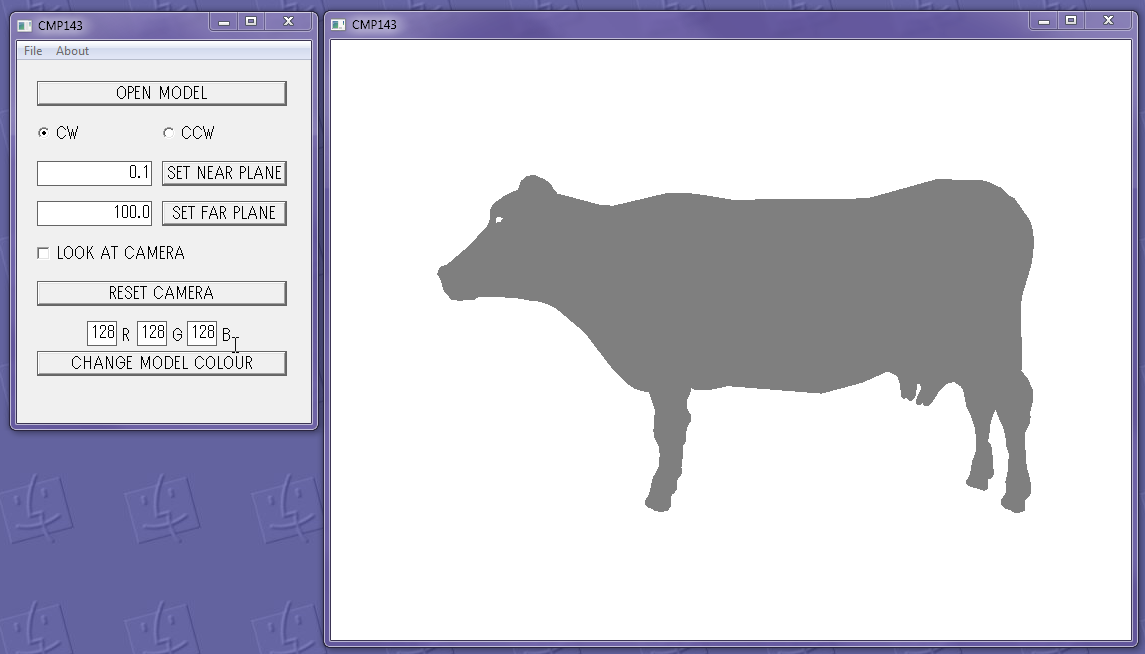
\includegraphics[scale=0.5]{3.png}
\end{center}
The Windows API was used to show the file picker dialog, the \texttt{ReadModelFile()} function reads the data from the input file, and then the model coefficients are created on the \texttt{BuildTriangles()} function, which creates a VAO with all the vertices from the input file and returns its id to the main function.

This assignment also uses the \texttt{matrices.h} library provided at the \textit{Fundamentals of Computer Graphics} laboratories to calculate some of the matrix transformations needed to display the object and control the camera.

\item[(b)] The camera can be translated using the W/S keys to go forward/backwards (camera Z axis), A/D keys to go left/right (camera X axis), and Q/Z keys to go up/down (camera Y axis).

From the starting position, this is the result after pressing W to translate the camera along its Z axis:
\begin{center}
	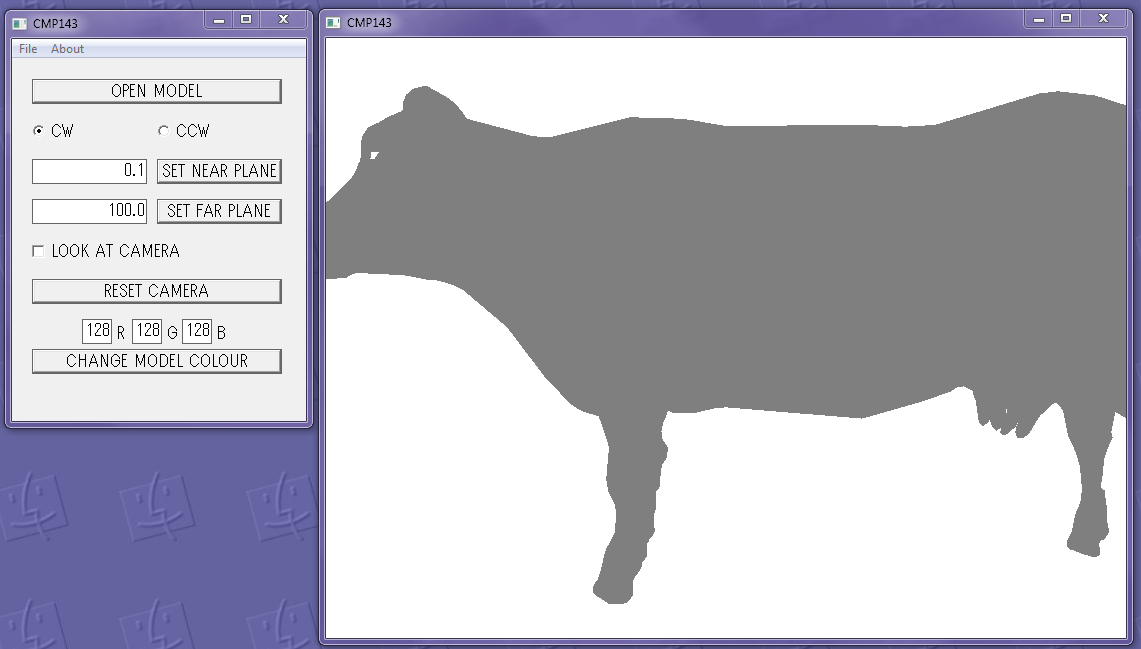
\includegraphics[scale=0.5]{4.png}
\end{center}
then, if pressed A to translate the camera along its X axis, this is the result:
\begin{center}
	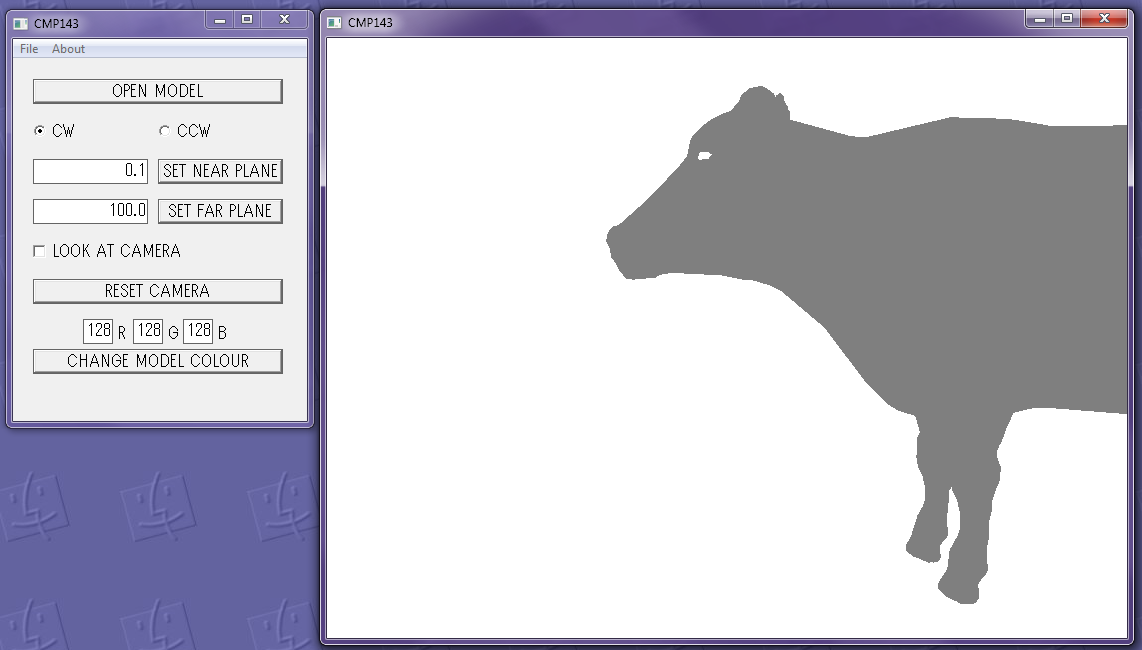
\includegraphics[scale=0.5]{5.png}
\end{center}
now, after pressing Q to translate the camera , this is the end result:
\begin{center}
	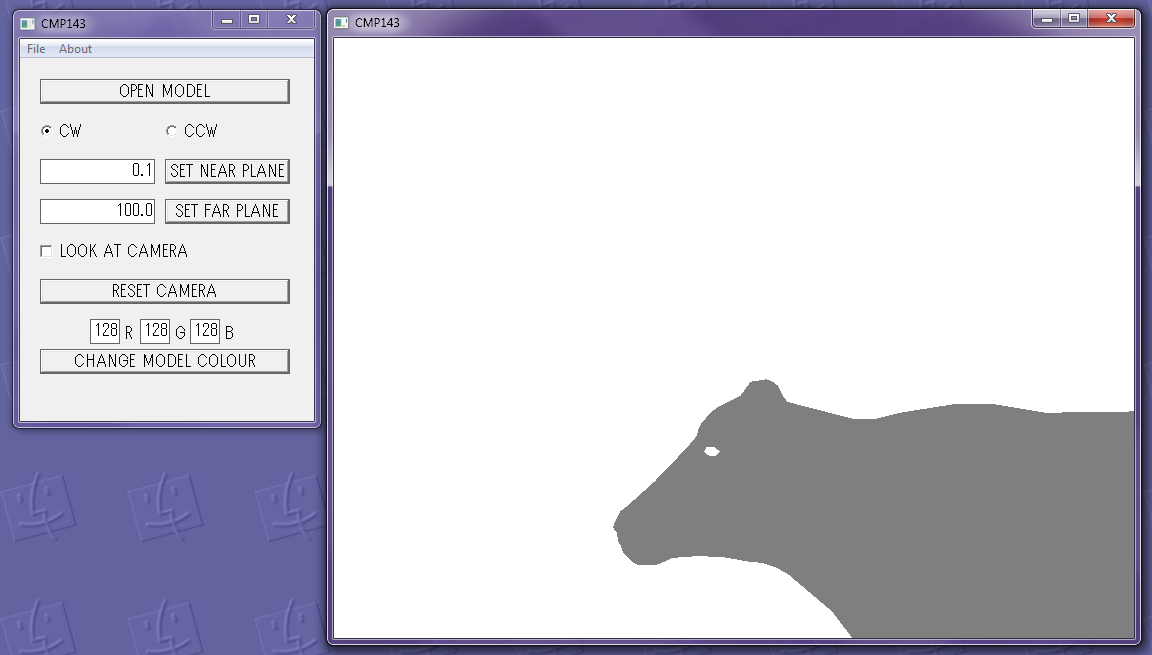
\includegraphics[scale=0.5]{6.png}
\end{center}
As it can be seen, the program is able to translate the camera along its three axes, and this translation is not dependent on the world coordinates, if the camera axes are rotated for example, the movement will occur along the camera axes, and not the world axes.

\item[(c)] The ``LOOK AT CAMERA'' checkbox can be checked to make the camera always look at the centre of the object while being translated.

When the look-at camera is translated along the Z axis, no rotation is needed as it only moves closer/farther from the object but the object continues being located at the centre of the camera.

When the look-at camera is translated along the X axis, it rotates a bit to continue focusing to the centre of the object, as expected. From the starting position, if the D key is pressed to translate the camera to the right, it rotates as well and the result is the following:
\begin{center}
	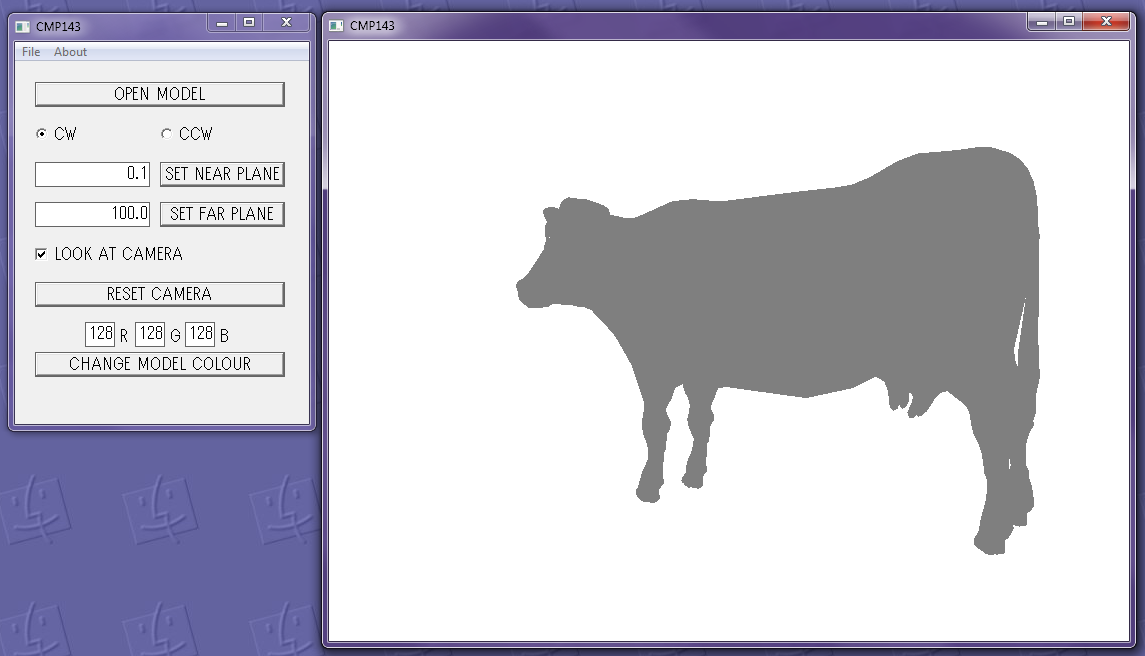
\includegraphics[scale=0.5]{7.png}
\end{center}
then, if the Z key is pressed the camera down, it also rotates to continue looking at the model, as shown below:
\begin{center}
	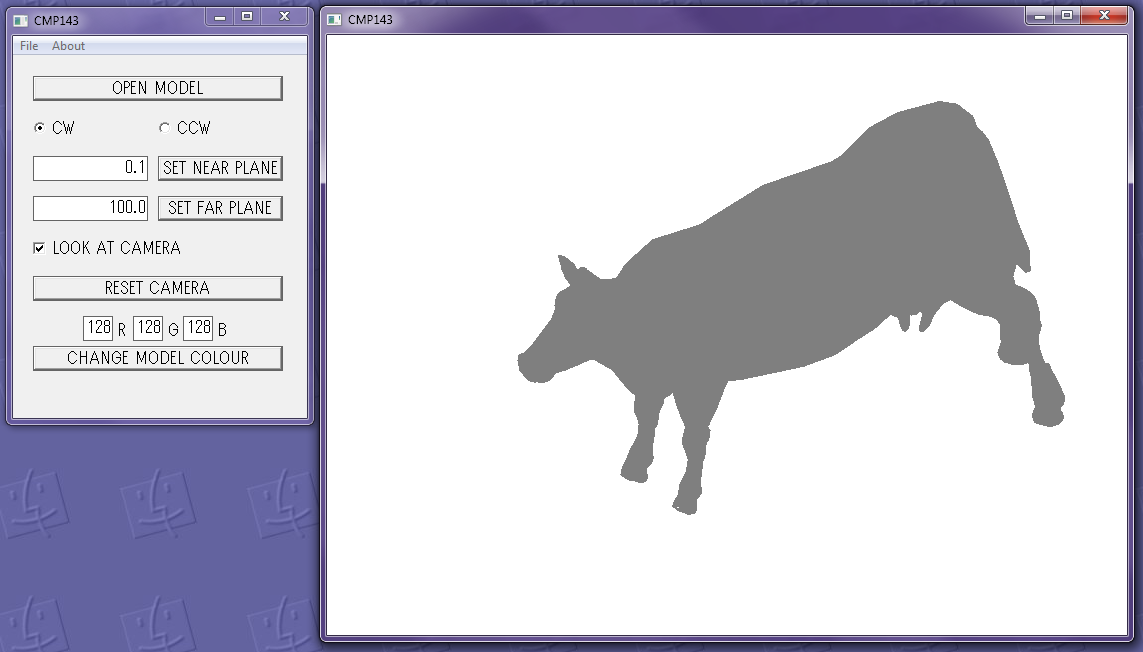
\includegraphics[scale=0.5]{8.png}
\end{center}

\item[(d)] The user can click and drag the cursor around the window to rotate the camera along its own axes.

From the starting position, this is the result if the cursor is clicked and dragged a bit towards the upper left corner of the window:
\begin{center}
	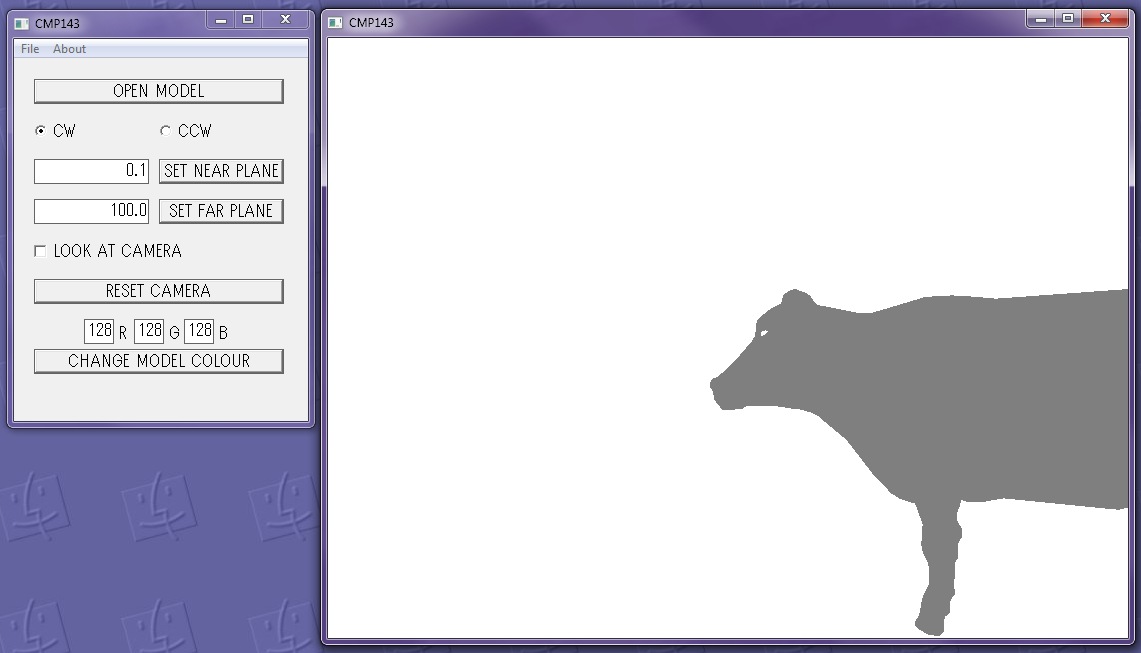
\includegraphics[scale=0.5]{9.png}
\end{center}
As it can be seen, the program is able to rotate the camera along its axes, and this rotation is not dependent on the world coordinates, if the camera axes are translated for example, the movement will occur along the camera axes, and not the world axes.

\item[(e)] There are two ways to reset the camera to its original position, the user can either press the `R' key on the keyboard, or click on the ``RESET CAMERA'' button on the interface. Both achieve the same result of setting the camera position and near/far plane values to the default values. This is the original position: 
\begin{center}
	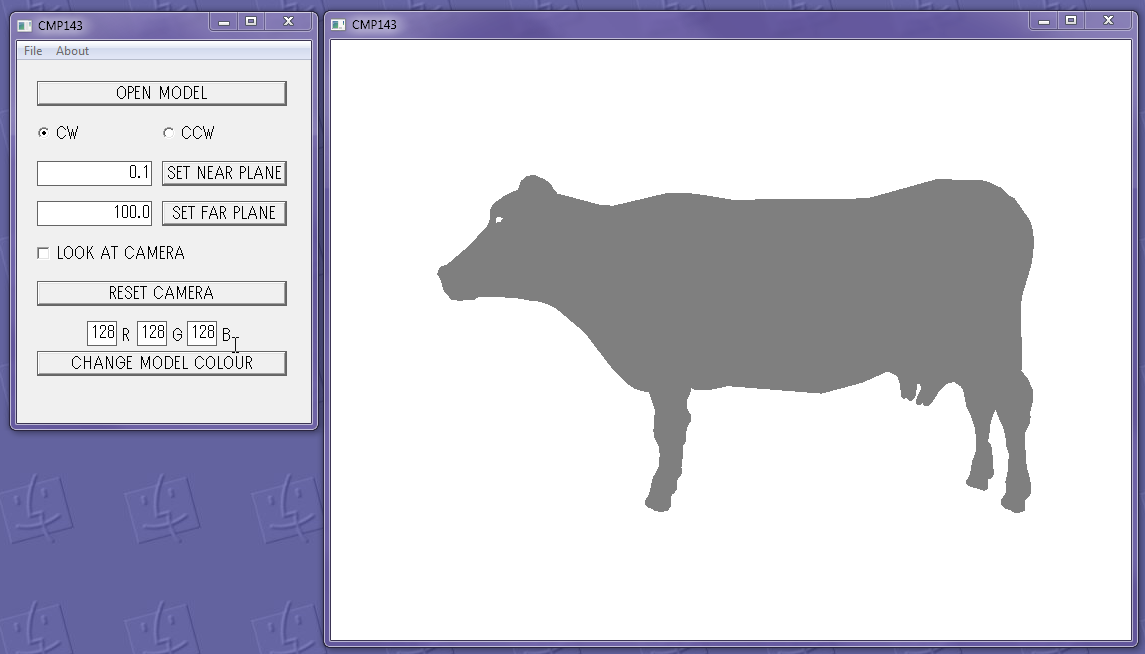
\includegraphics[scale=0.5]{3.png}
\end{center}

\item[(f)] The ``CW / CCW'' toggle is used to change the orientation of the vertices from the model, since there are no light effects, it's not possible to notice much difference at first glance, but with the cow model on the original position the eyes position will appear to have changed depending on the mode, as shown below:
\begin{center}
	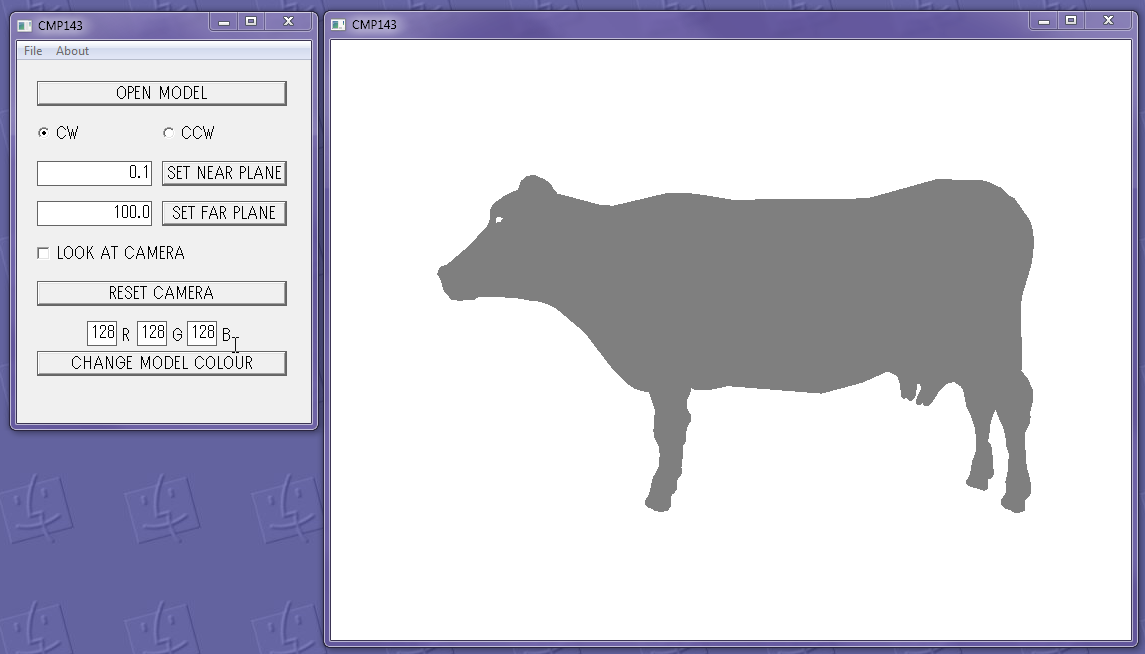
\includegraphics[scale=0.5]{3.png}
	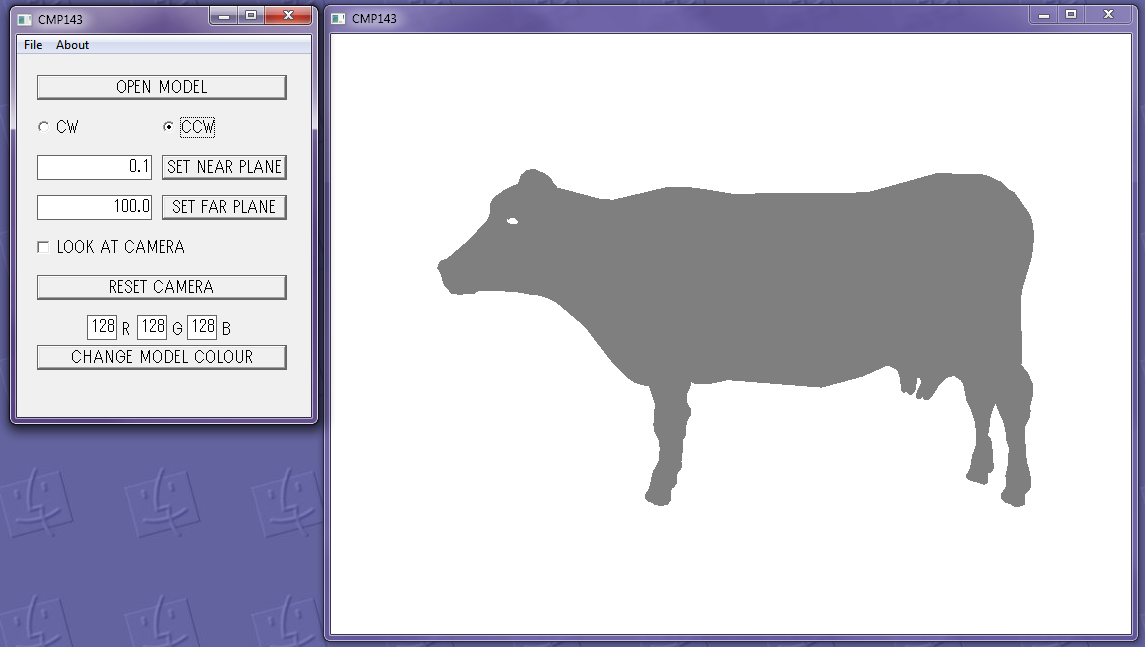
\includegraphics[scale=0.5]{10.png}
\end{center}

\item[(g)] The values for the near and far planes can be changed from the interface on the left window. These are some of the results achieved by changing the values to cut the cow at about half first from the far plane and then at the near plane (using the CCW mode to be able to better visualize the result):
\begin{center}
	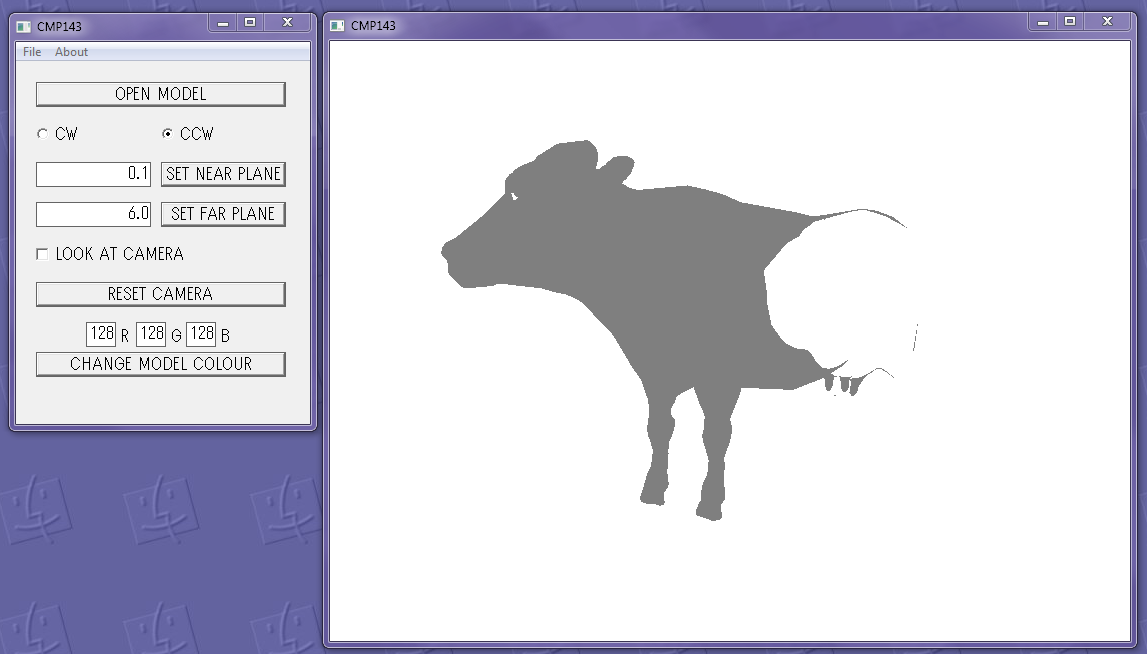
\includegraphics[scale=0.5]{11.png}
	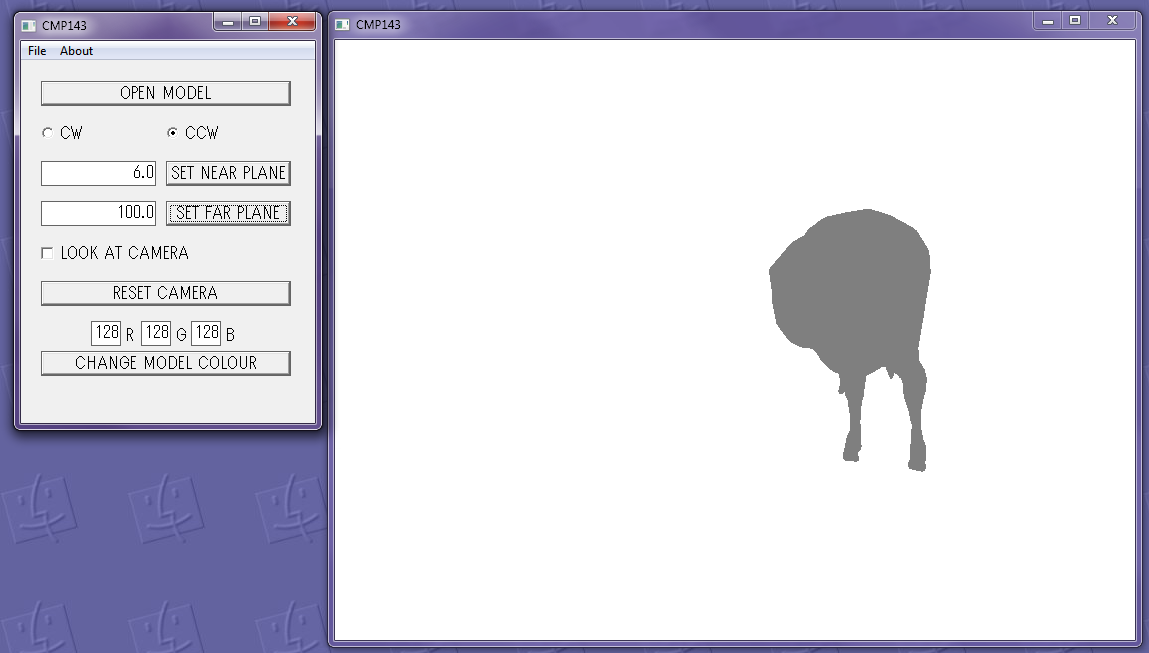
\includegraphics[scale=0.5]{12.png}
\end{center}

\item[(h)] The R, G and B values from the model can be changed on the interface by typing the values on the corresponding textboxes, the values must be between 0 and 255, and clicking the ``CHANGE MODEL COLOUR'' button. These are some of the results obtained:
\begin{center}
	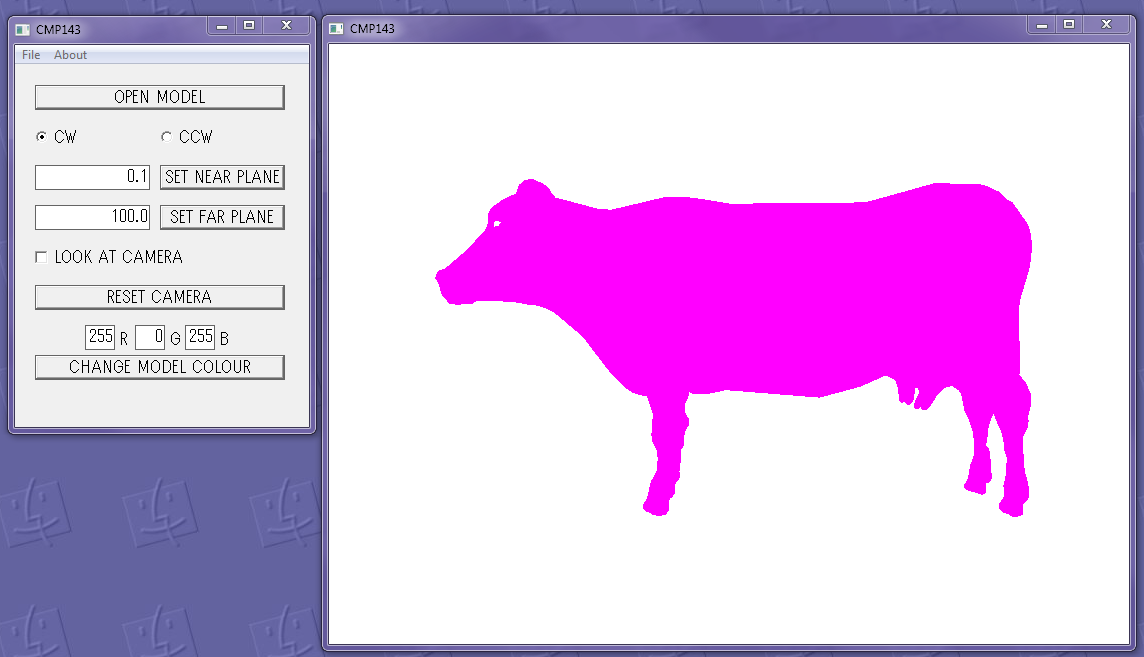
\includegraphics[scale=0.5]{13.png}
	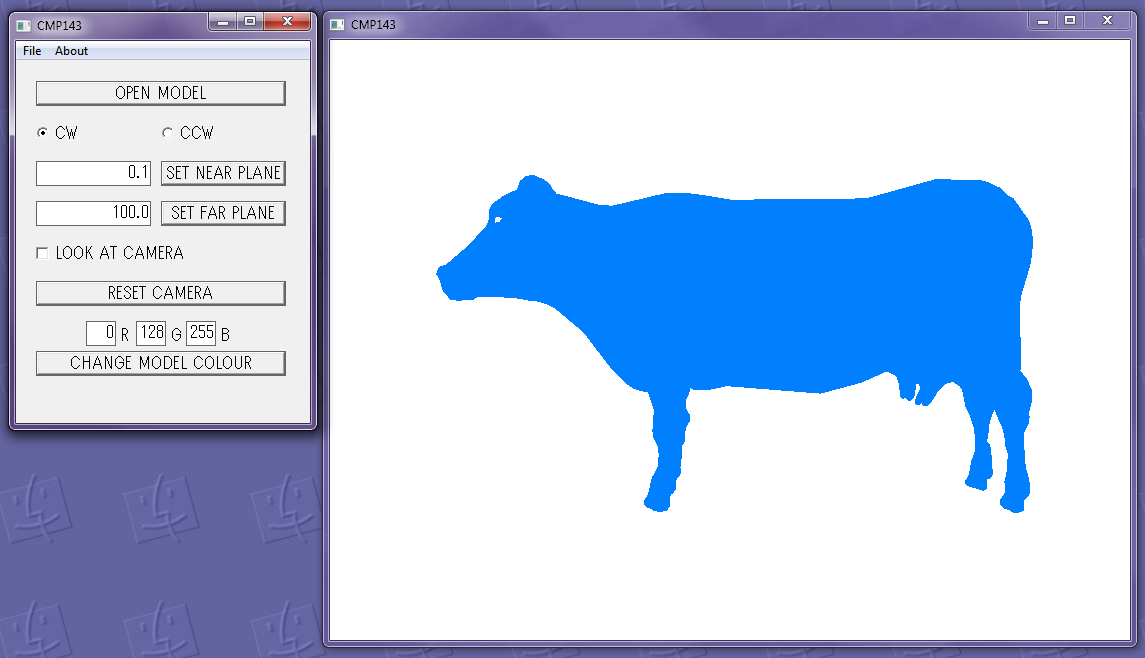
\includegraphics[scale=0.5]{14.png}
\end{center}
\end{itemize}

The source code is included with this report, and it's also available at https://github.com/beckJJ/CMP143

\end{document}